\documentclass[tikz,border=5pt]{standalone}
\usepackage{pgfplots}
\pgfplotsset{compat=1.18}
\usepackage{fontspec}
\setsansfont{SourceSansPro}[
  Path = /usr/local/texlive/2024/texmf-dist/fonts/opentype/adobe/sourcesanspro/,
  UprightFont = SourceSansPro-Regular.otf,
  BoldFont = SourceSansPro-Bold.otf,
  ItalicFont = SourceSansPro-RegularIt.otf,
  BoldItalicFont = SourceSansPro-BoldIt.otf,
  Scale = 1.0
]
\usetikzlibrary{positioning}
\usepackage{xcolor}
\definecolor{primaryblue}{HTML}{012169}
\definecolor{primarygold}{HTML}{B9975B}
\definecolor{highlightyellow}{HTML}{F2A900}
\definecolor{lightbg}{HTML}{E8EDF5}
\definecolor{jet}{HTML}{1A1A1A}
\definecolor{positivegreen}{HTML}{15803D}
\definecolor{negativered}{HTML}{B91C1C}
\newcommand{\hi}[1]{{\bfseries\color{primaryblue}#1}}
\begin{document}
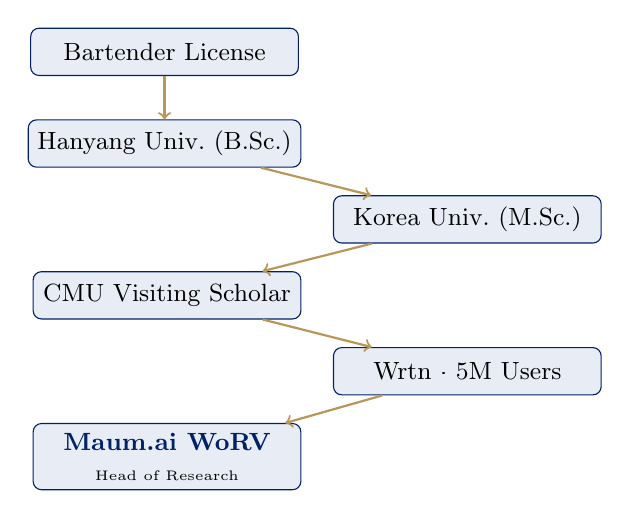
\begin{tikzpicture}[
  node distance=0.55cm,
  box/.style={draw=primaryblue, rounded corners=3pt, fill=lightbg,
              minimum width=3.4cm, minimum height=0.6cm,
              font=\small, align=center},
  arrow/.style={->, thick, color=primarygold}
]
  \node[box] (bar)  {Bartender License};
  \node[box, below=of bar]  (han)  {Hanyang Univ.\ (B.Sc.)};
  \node[box, below right=0.35cm and 0.4cm of han] (kor)  {Korea Univ.\ (M.Sc.)};
  \node[box, below left=0.35cm and 0.4cm of kor]  (cmu)  {CMU Visiting Scholar};
  \node[box, below right=0.35cm and 0.4cm of cmu] (wrtn) {Wrtn · 5M Users};
  \node[box, below left=0.35cm and 0.4cm of wrtn] (maum) {\hi{Maum.ai WoRV}\\
        \tiny Head of Research};

  \draw[arrow] (bar)  -- (han);
  \draw[arrow] (han)  -- (kor);
  \draw[arrow] (kor)  -- (cmu);
  \draw[arrow] (cmu)  -- (wrtn);
  \draw[arrow] (wrtn) -- (maum);
\end{tikzpicture}
\end{document}
